% Chapter 1

\chapter{Resultados} % Main chapter title

\label{Cap_Res} % For referencing the chapter elsewhere, use \ref{Chapter1} 

----------------------------------------------------------------------------

En los dos experimentos realizados, los patrones de respuesta identificados como parte del Efecto Espejo, tanto en la emisión de juicios de detección como en la escala de confianza, se encontraron en más de tres cuartas partes de los participantes. De los 20 participantes en el Experimento 1, 17 mostraron evidencia del efecto espejo en la emisión de juicios de detección y 18 en términos de escalas de confianza; en el caso del Experimento 2, 19 de los 21 participantes mostraron evidencia del Efecto Espejo en ambas tareas. 


We had 20 and 21 participants on Experiments 1 and 2 respectively. In both cases, we found evidence for the Mirror Effect in at least 85\% of the participants. In Experiment 1, we had 17 cases showing the Mirror Effect pattern within the hit and false alarm rates and 18 in terms of Confidence Ratings. In Experiment 2 we had 19 participants showing the Mirror Effect in both patterns of response. All these proportions were statistically significant when we apply a simple Binomial Test (p=0.0025 and p=0.0004, for Experiment 1, and p=0.0002 for Experiment 2).

\section{Las condiciones propuestas difieren en su discriminabilidad}



\begin{figure}[th]
\centering
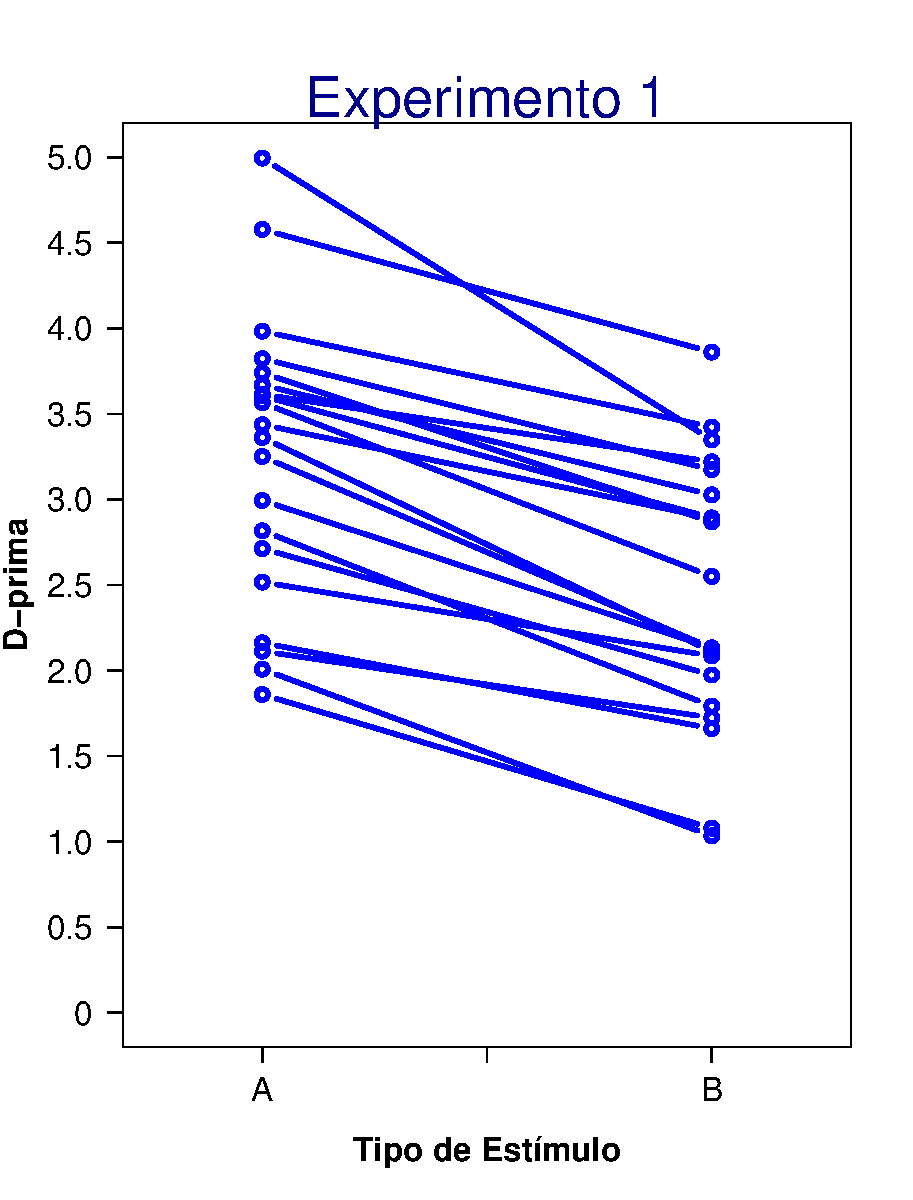
\includegraphics[width=0.40\textwidth]{Figures/Diff_D_E1} 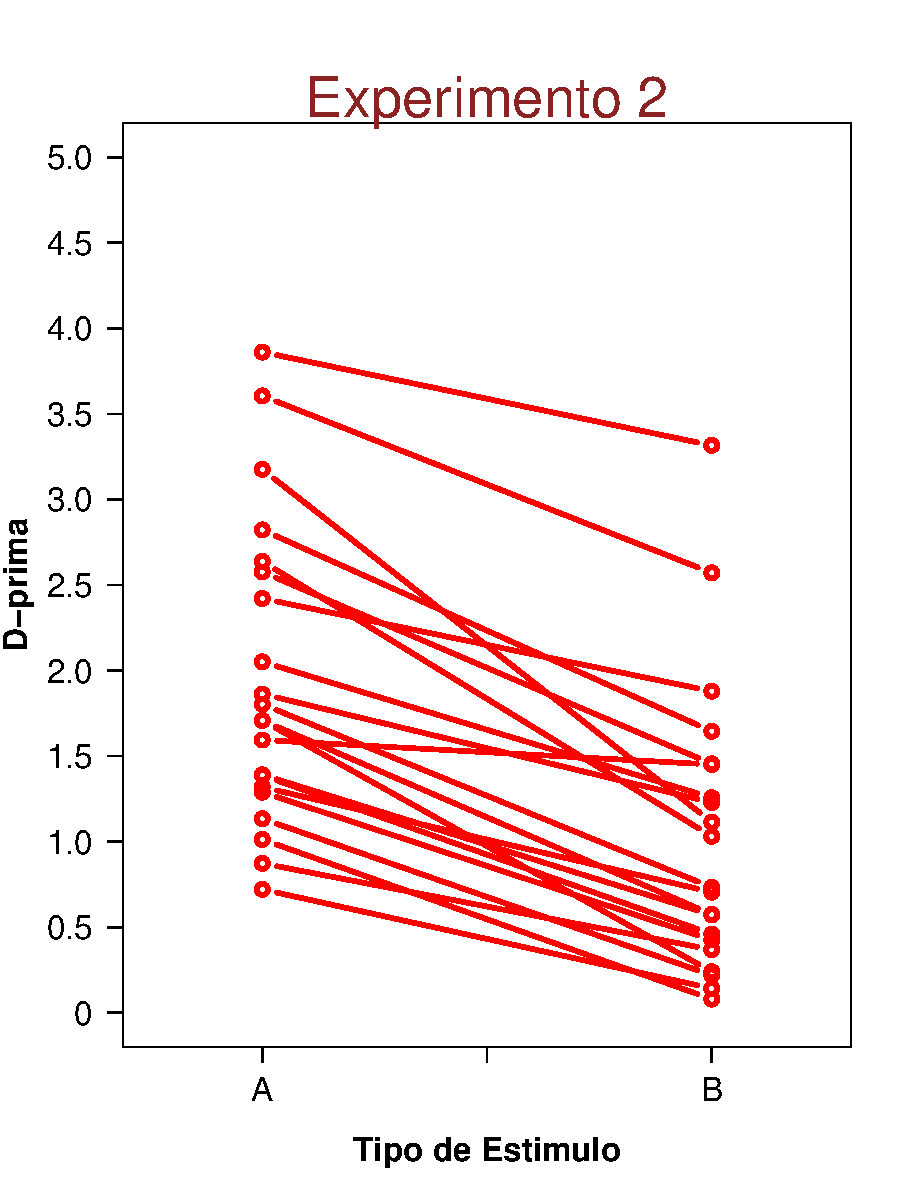
\includegraphics[width=0.40\textwidth]{Figures/Diff_D_E2}
%\decoRule
\caption[Diferencias en Discriminabilidad (Comprobando diferencias entre condiciones)]{ }
\label{fig:Diff_D}
\end{figure}

%----------------------------------------------------------------------------------------

\section{Diferencias en las Tasas de Hits y Falsas Alarmas}

\begin{figure}[th]
\centering
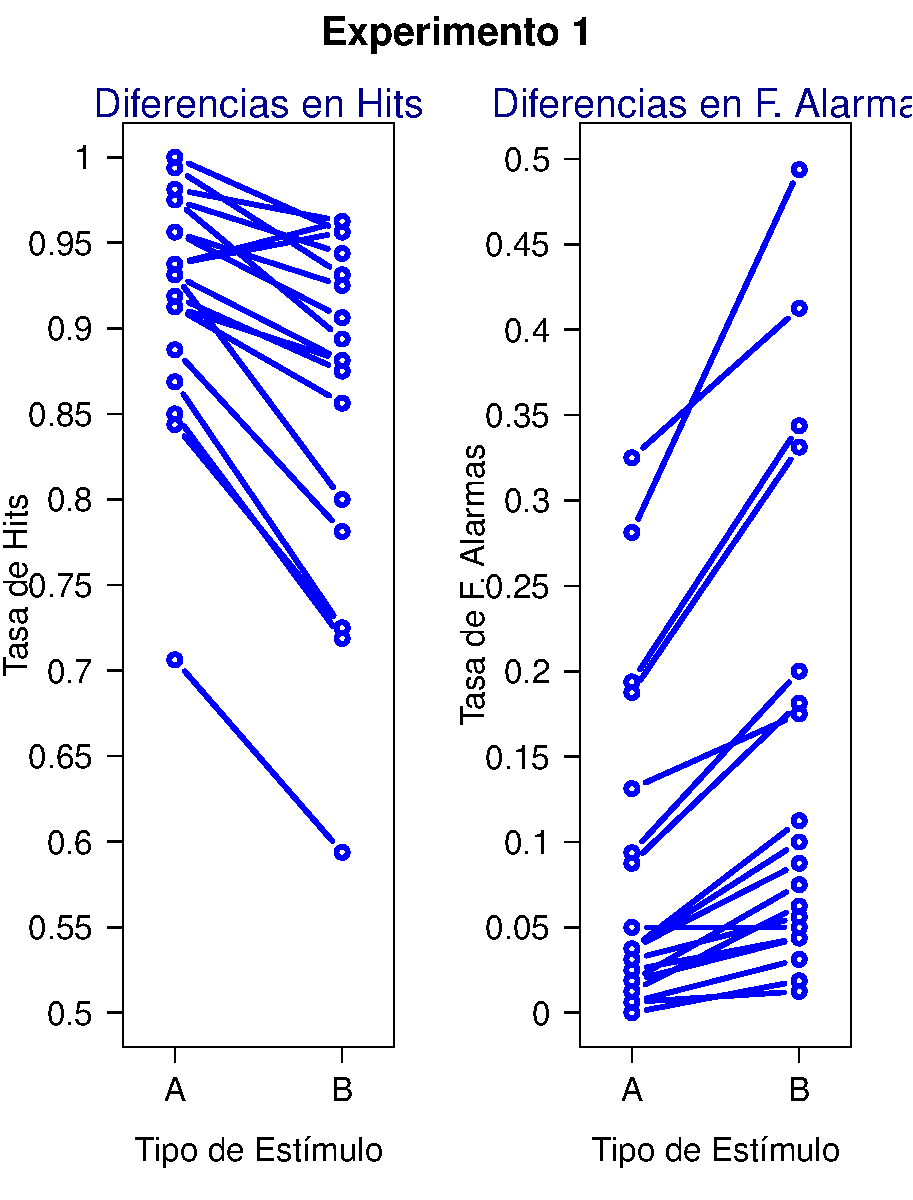
\includegraphics[width=0.35\textwidth]{Figures/Diff_Rate_E1} 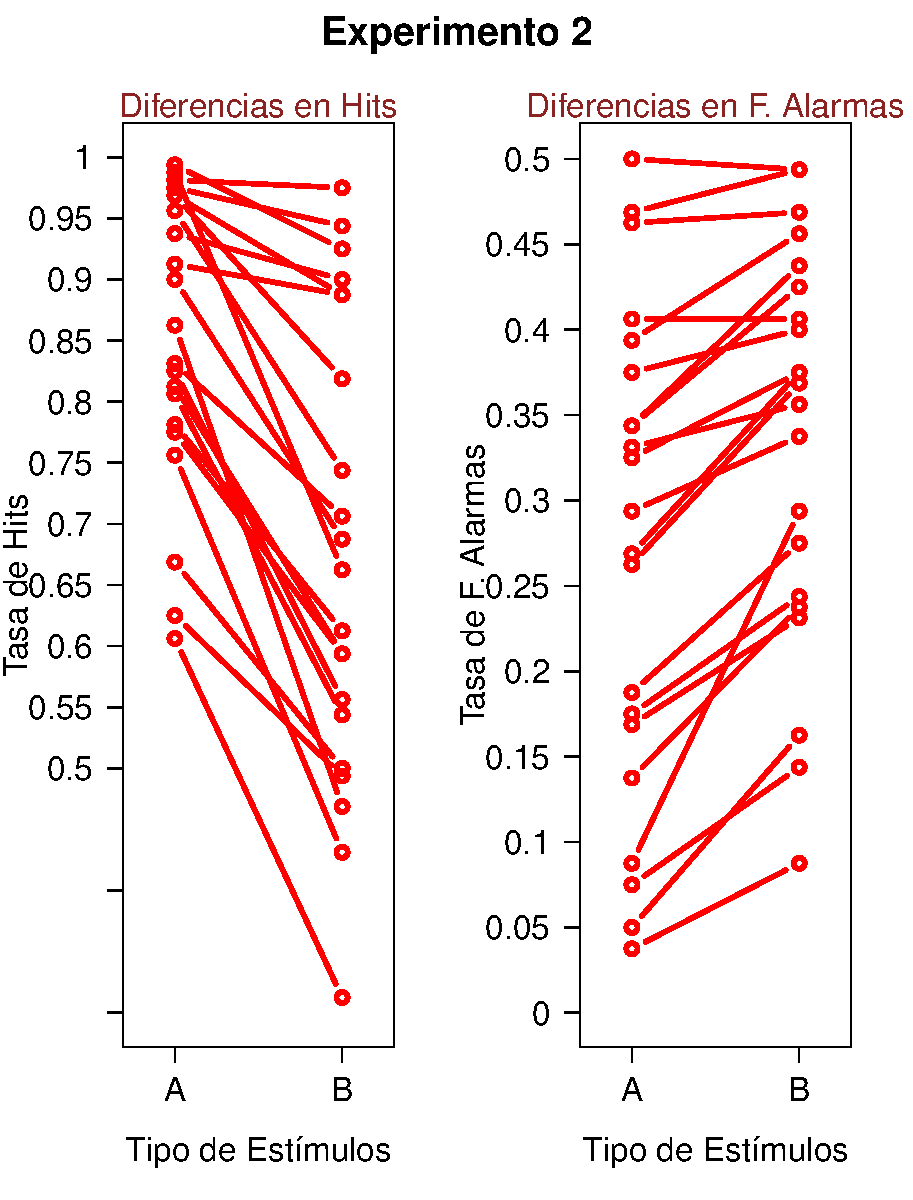
\includegraphics[width=0.35\textwidth]{Figures/Diff_Rate_E2}
%\decoRule
\caption[Diferencias en Tasas (Comprobando diferencias entre condiciones)]{Comparación intrasujeto de}
\label{fig:Diff_Rate}
\end{figure}
